
%%%%%%%%%%%%%%%%%%%%%%% file typeinst.tex %%%%%%%%%%%%%%%%%%%%%%%%%
%
% This is the LaTeX source for the instructions to authors using
% the LaTeX document class 'llncs.cls' for contributions to
% the Lecture Notes in Computer Sciences series.
% http://www.springer.com/lncs       Springer Heidelberg 2006/05/04
%
% It may be used as a template for your own input - copy it
% to a new file with a new name and use it as the basis
% for your article.
%
% NB: the document class 'llncs' has its own and detailed documentation, see
% ftp://ftp.springer.de/data/pubftp/pub/tex/latex/llncs/latex2e/llncsdoc.pdf
%
%%%%%%%%%%%%%%%%%%%%%%%%%%%%%%%%%%%%%%%%%%%%%%%%%%%%%%%%%%%%%%%%%%%


\documentclass[runningheads,a4paper]{llncs}

\usepackage{listings}
\usepackage{amssymb}
\usepackage{graphicx}
\usepackage{longtable}
\usepackage{url}
\usepackage{xcolor}
\usepackage{acro}


\newcommand{\keywords}[1]{\par\addvspace\baselineskip
\noindent\keywordname\enspace\ignorespaces#1}
\usepackage{nameref}
\acsetup{first-style=short}

% Abbreviations
\DeclareAcronym{dp}{short = DP, long = Draw Pile Module, class = abbrev}
\DeclareAcronym{fp}{short = FP, long = Foundation Pile Module, class = abbrev}
\DeclareAcronym{tp}{short = TP, long = Tableau Pile Module, class = abbrev}
\DeclareAcronym{p}{short = P, long = Player Module, class = abbrev}
\DeclareAcronym{pb}{short = PB, long = Player Bot Module, class = abbrev}
\DeclareAcronym{fifo}{short = FIFO, long = First In First Out (Queue), class = abbrev}
\DeclareAcronym{lifo}{short = LIFO, long = Last In First Out (Stack), class = abbrev}
\DeclareAcronym{gui}{short = GUI, long = Graphical User Interface, class = abbrev}

% Nomenclature
\DeclareAcronym{card}{short = card, long = (In the Petri Net context) A token with a color which represents a card in the deck., class = nomencl}
\DeclareAcronym{command}{short = command, long = A token with a color which represents a turn or movement command., class = nomencl}

\newcommand{\GPenSIM}{../GPenSIM}
\definecolor{matlabcomment}{RGB}{34,139,34}
\definecolor{matlabstring}{RGB}{160,32,240}
\definecolor{matlabkeyword}{RGB}{0,0,255}
\lstdefinestyle{matlabcode}{
	language=Matlab,
	frame=single,
	%caption={\protect\filename@parse{\lstname}\protect\filename@base},
	caption=\lstname,
	stringstyle=\color{matlabstring},
	keywordstyle=\color{matlabkeyword},
	commentstyle=\color{matlabcomment},
	basicstyle=\fontsize{6}{7}\selectfont,%\tiny
	breaklines=true,
	numbers=left
}

\begin{document}
\mainmatter  % start of an individual contribution
% first the title is needed
\title{DAT530\\Discrete Simulation and Performance Analysis\\Final Project\\Solitaire game strategy}
% a short form should be given in case it is too long for the running head
\titlerunning{DAT530 - Final Project}
\author{Racin W. Nygaard}
\authorrunning{DAT530 - Final Project - Solitaire game strategy}
% (feature abused for this document to repeat the title also on left hand pages)
\institute{Universitetet i Stavanger}

\toctitle{Abstract}
\tocauthor{ }
\maketitle
	


\begin{abstract}
This project is such and such... +++

\end{abstract}

\setcounter{tocdepth}{2}
\tableofcontents

\listoffigures
\listoftables
\printacronyms[name=Abbreviations,include-classes=abbrev]
\printacronyms[name=Nomenclature,include-classes=nomencl]
\section{Introduction}
This project aims to study the popular card game, Solitaire[Site]. Solitaire is bundled with most Windows[Site] installations, as well as being available for free on several sources. It is also easy to play the game with a physical card deck. A detailed explaination of the games rules can be found in the next chapter, Solitaire Rules[REF]
\newline
Since the game utilizes all 52 cards of the deck, the number of possible initial game states is 52!, which is a very high number. A large number of these inital game states can be merged, as they offer no difference in the difficulty to solve. Some of these intial states are unsolvable, but even given a solvable game state, one often find oneself in an unsolvable game state, due to certain actions in the game are non-reversible,. There has been attempts to find the distribution of solvable and unsolvable initial game states [ref]. This is roughly 75 percent are solvable, however the study also shows that only 35 percent of the games are won by an experienced player.
\newline
This project contains a complete model of the game, a GUI to play the game, and a basic bot to simulate user actions. 

\subsection{Solitaire Rules}


Finite State Machine ?


\section{Method and Design}
\label{sec:2_method_and_design}
\subsection{Naming Policy}
%\begin{table}
%	\caption{Places}
%	\begin{tabular}{|l|l|l|l|}
%		\hline
%		 & Name & Module & Usage \\
%		\hline

%		21 & tMC\_DP\_Move\_Siphon    &  &  \\ \hline
%		22 & tMC\_FP\_Move\_Siphon    &  &  \\ \hline
%		23 & tMC\_Out\_Buffer\_Siphon &  &  \\ \hline
%		24 & tMC\_TP\_Move\_Siphon    &  &  \\ \hline
%		25 & tMC\_TP\_Turn\_Siphon    &  &  \\ \hline
%		26 & tPBe\_DP\_Move           &  &  \\ \hline
%		27 & tPBe\_DP\_Turn           &  &  \\ \hline
%		28 & tPBe\_FP\_Move           &  &  \\ \hline
%		29 & tPBe\_TP\_Move           &  &  \\ \hline
%		30 & tPBe\_TP\_Turn           &  &  \\ \hline
%		31 & tPBi\_Gen                &  &  \\ \hline
%		32 & tPBi\_Siphon             &  &  \\ \hline
%		33 & tPe\_DP\_Move            &  &  \\ \hline
%		34 & tPe\_DP\_Turn            &  &  \\ \hline
%		35 & tPe\_FP\_Clubs\_Move     &  &  \\ \hline
%		36 & tPe\_FP\_Diamonds\_Move  &  &  \\ \hline
%		37 & tPe\_FP\_Hearts\_Move    &  &  \\ \hline
%		38 & tPe\_FP\_Spades\_Move    &  &  \\ \hline
%		39 & tPe\_TP\_1\_Move         &  &  \\ \hline
%		40 & tPe\_TP\_1\_Turn         &  &  \\ \hline
%		41 & tPe\_TP\_2\_Move         &  &  \\ \hline
%		42 & tPe\_TP\_2\_Turn         &  &  \\ \hline
%		43 & tPe\_TP\_3\_Move         &  &  \\ \hline
%		44 & tPe\_TP\_3\_Turn         &  &  \\ \hline
%		45 & tPe\_TP\_4\_Move         &  &  \\ \hline
%		46 & tPe\_TP\_4\_Turn         &  &  \\ \hline
%		47 & tPe\_TP\_5\_Move         &  &  \\ \hline
%		48 & tPe\_TP\_5\_Turn         &  &  \\ \hline
%		49 & tPe\_TP\_6\_Move         &  &  \\ \hline
%		50 & tPe\_TP\_6\_Turn         &  &  \\ \hline
%		51 & tPe\_TP\_7\_Move         &  &  \\ \hline
%		52 & tPe\_TP\_7\_Turn         &  &  \\ \hline

%	\end{tabular}
%\end{table}
%\begin{table}
%	\caption{Places used in Draw Pile}
%	\begin{tabular}{|l|l|l|}
%		\hline
%		& Name & Description \\
%		\hline
%		15 & pMC\_DP\_Move             &  \\ \hline
%		16 & pMC\_DP\_Turn             &  \\ \hline
%		17 & pMC\_FP\_Move             &  \\ \hline
%		18 & pMC\_Out\_Buffer          &  \\ \hline
%		19 & pMC\_TP\_Move             &  \\ \hline
%		20 & pMC\_TP\_Turn             &  \\ \hline
%		21 & pPB\_Cmd                  &  \\ \hline

%	\end{tabular}
%\end{table}
\subsection{Overall Design}

\begin{figure}
	\label{fig:full_horizontal}
	\begin{center} % Left, Bottom, Right, Top
		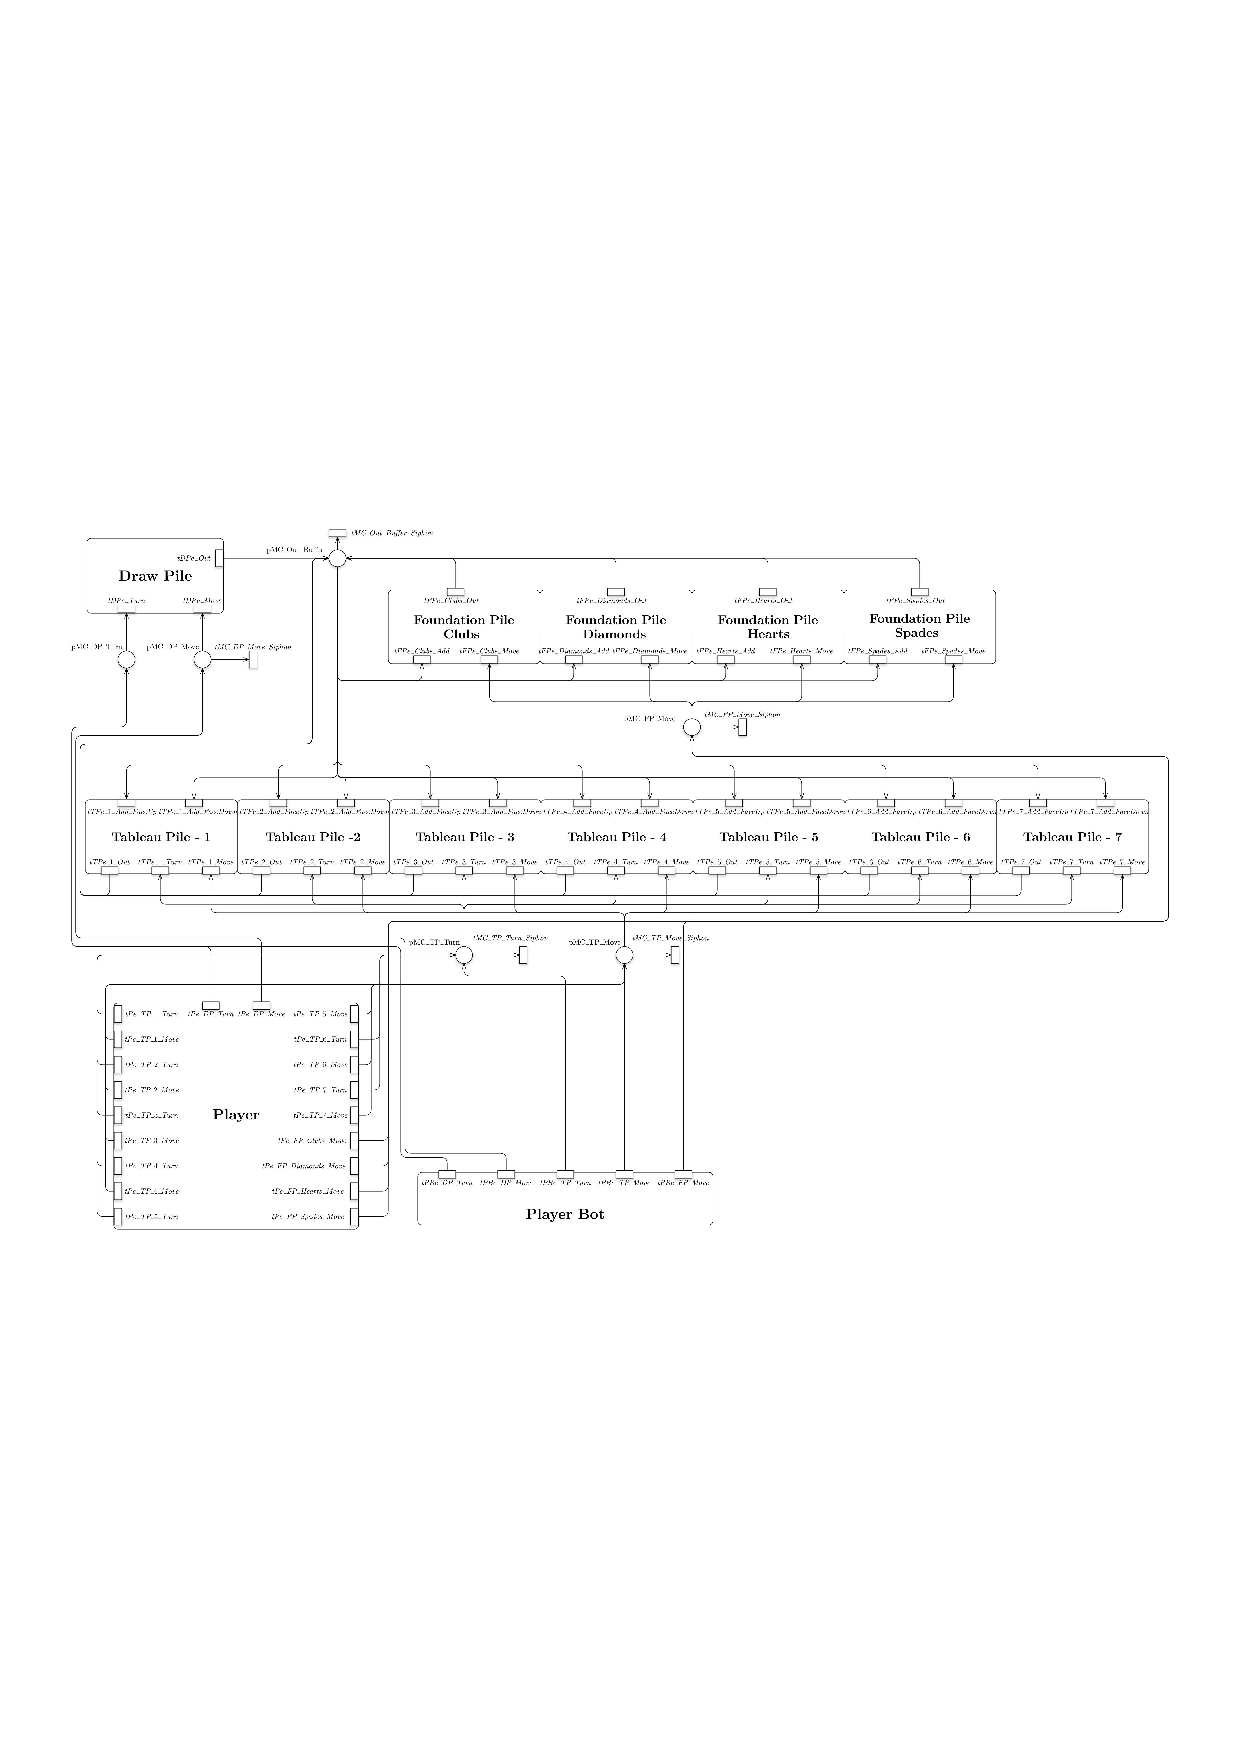
\includegraphics[trim=250 260 230 330,scale=1.1]{images/overallViewPdf}
	\end{center}
	\caption{The complete model - Without the internal components of the modules.}
\end{figure}


\begin{figure}
	\label{fig:full_vertical}
	 % Left, Bottom, Right, Top
	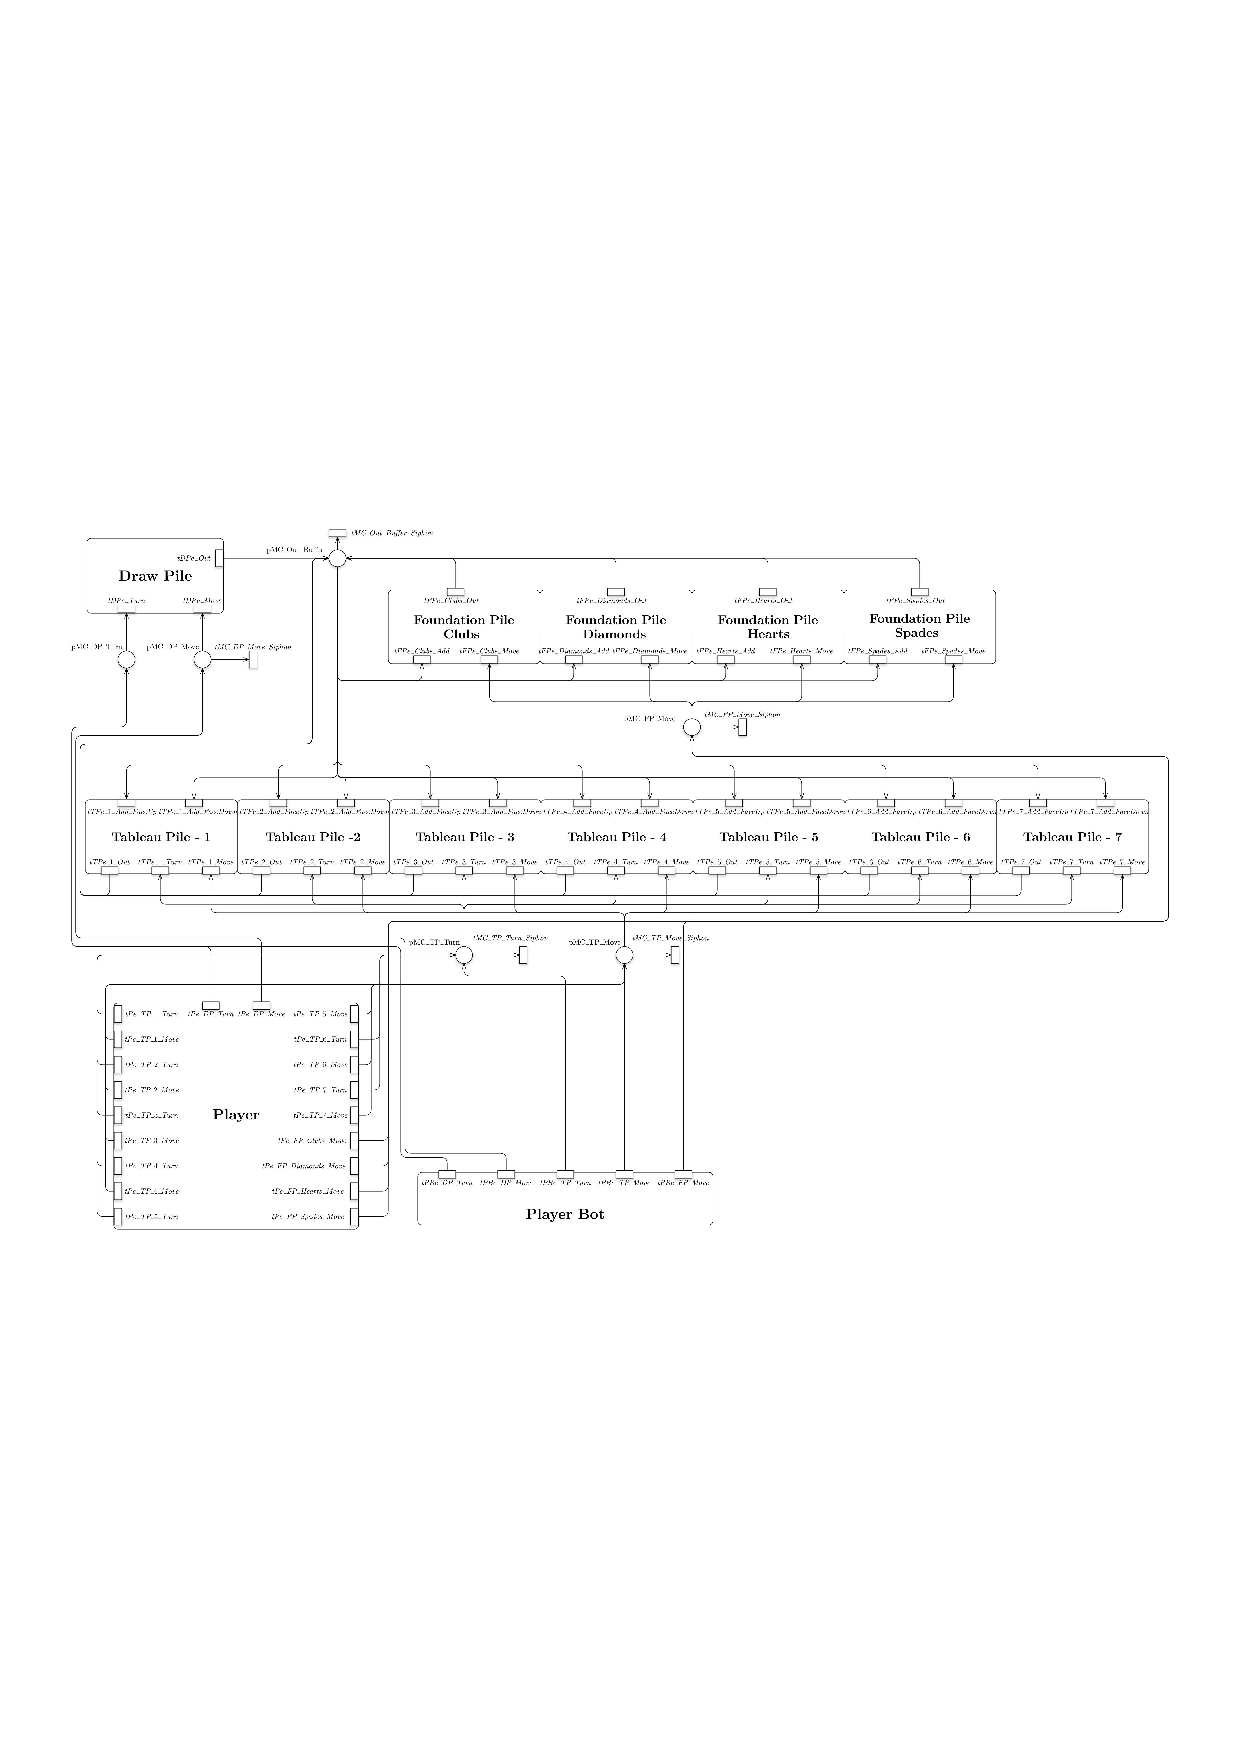
\includegraphics[trim=40 100 100 310,angle=90,scale=1.4]{images/overallViewPdf}
	\caption{The complete model - Without the internal components of the modules.}
\end{figure}
The model developed is pretty large, and contains 94 transition and 42 places. It is developed using the modualar approach, and encompasses 6 different modules. Some of the modules are duplicated, with the only difference being the names of the transitions and places.
\newline

\subsection{Draw Pile Module}

\begin{figure}
	\begin{center}
		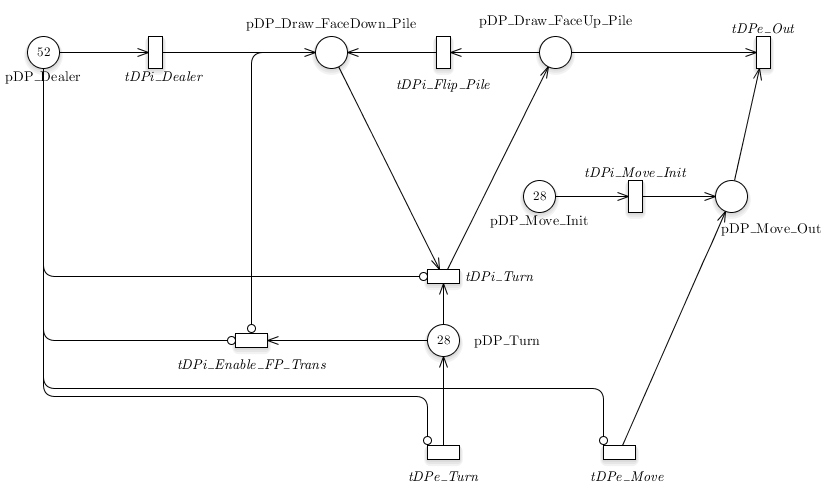
\includegraphics[width=\textwidth]{images/drawPile}
		\caption{Draw Pile Module}
		\label{fig:draw_pile}
	\end{center}
\end{figure}
The Draw Pile module is depicted in figure \ref{fig:draw_pile}, and has several key responsibilities, once of which is to do the initial dealing of cards. In order to preserve the correctness of the gameplay, external input is not allowed during this phase. When first running the model, all the initial tokens of \verb!pDP_Dealer! will be sent to \verb!tDPi_Dealer!. This transition will give each token a color which represents a \ac{card} in the deck. Possible colors are initially stored in the cell \verb!global_info.DECK!. If \verb!global_info.RANDOM_DECK! is set, a random permutation of the colors will be given to the tokens. By having \verb!global_info.RANDOM_DECK! set to false, it is possible to run analytics which require that the cards are dealt equally each time.
\newline

After all tokens are given a color, \verb!tDPi_Turn! will be enabled. This transition will move cards from the pile which represents face-down cards, \verb!pDP_Draw_FaceDown_Pile! to the one representing face-up cards, \verb!pDP_Draw_FaceUp_Pile!. This transition will fire as many times as the length of \verb!global_info.INITIAL_DEAL_MOVE!, which is 28 in a normal game. This is not something that would be done if the game where played with physical cards, as they would just be dealt without turning them. In this model however, this is required so that existing logic could be re-used.
\newline

Concurrently to the firing of \verb!tDPi_Turn!, the transition \verb!tDPi_Move_Init! will fire an equal amount of times. The transition will give each of the tokens in \verb!pDP_Move_Init! a color which represents to which tableau pile the \ac{card} should be moved to. The color given to each token is augmented by the cell, \verb!global_info.INITIAL_DEAL_MOVE!. An example of a color given is \emph{Move:\ac{tp}1:\ac{dp}} which means; \textit{Moving a card from source DP to destination \ac{tp}1}. Every time a \ac{card} reaches its destined tableau pile, the variable \verb!global_info.CARDS_DEALT! will be incremented by one in \verb!COMMON_POST!. Once it becomes equal to the length of \verb!global_info.INITIAL_DEAL_MOVE!, the initial dealing phase is over, and the normal phase starts.
\newline

During the normal phase, external input is allowed. The first input of the Draw Pile Module is \verb!tDPe_Move!. This transition has an pre-processor file, which makes it only fire if there are tokens in \verb!pDP_Draw_FaceUp_Pile!. Additionally, the Player and Player Bot modules ensures that the enabling token has color on the format \textit{Move:(destination):\ac{dp}}.
\lstinputlisting[style=matlabcode,caption=tDPe\_Move\_pre.m,label=lst:tDPe_Move_pre]{\GPenSIM/tDPe_Move_pre.m}

The second input, \verb!tDPe_Turn! is used to used to simply move cards from the face-down pile to the face-up pile during the normal phase. An interesting thing about this is that once all the cards are in the face-up pile, the next time one attempts to turn a \ac{card}, all cards should be moved back to the face-down pile in \ac{lifo} style, just as they would if you simply flip the deck of cards around in real-life. 
\newline
This is accomplished by the transitions \verb!tDPi_Flip_Pile! and \verb!tDPi_Enable_DP_Trans!. The \verb!tDPi_Enable_FP_Trans! is actually an siphon, and becomes enabled once \verb!pDP_Draw_FaceDown_Pile! is empty, and there is an active turn action on-going so that \verb!pDP_Turn! has at least one token. The transition has one post-processor file, shown in listing \ref{lst:tDPi_Enable_FP_Trans_post}. Given that there are actually any tokens left in \verb!pDP_Draw_FaceUp_Pile! it will set the global flag, \verb!global_info.DP_Flip_Pile_Running! to \verb!true!, if there are no tokens in the face-up pile, it will simply release the \verb!playerAction! resource. The use of resources is discussed further in chapter \ref{sec:3_Resources}. The reason for not having an arc directly from the face-up pile is due to this transition being a siphon, so the \ac{card} would be removed from the game if it fired.
\lstinputlisting[style=matlabcode,caption=tDPi\_Enable\_FP\_Trans\_post.m,label=lst:tDPi_Enable_FP_Trans_post]{\GPenSIM/tDPi_Enable_FP_Trans_post.m}
Once \verb!global_info.DP_Flip_Pile_Running! is set to \verb!true! and there are tokens in \verb!pDP_Draw_FaceUp_Pile!, the transition \verb!tDPi_Flip_Pile! will start firing. The pre-processor file is listed in \ref{lst:tDPi_Flip_Pile_pre}, and will keep selecting the latest arrived \ac{card} from \verb!pDP_Draw_FaceUp_Pile! and fire. In the post-processor file, listed in \ref{lst:tDPi_Flip_Pile_post}, it will check for the length of the face-up pile, once it becomes empty it will set the flag \verb!global_info.DP_Flip_Pile_Running! to \verb!false!, and the cards have been successfully turned around.
\lstinputlisting[style=matlabcode,caption=tDPi\_Flip\_Pile\_pre.m,label=lst:tDPi_Flip_Pile_pre]{\GPenSIM/tDPi_Flip_Pile_pre.m}
\lstinputlisting[style=matlabcode,caption=tDPi\_Flip\_Pile\_post.m,label=lst:tDPi_Flip_Pile_post]{\GPenSIM/tDPi_Flip_Pile_post.m}

Lastly, there is the \verb!tDPe_Out! transition. This is the only external output of the module. When enabled, its pre-processor will take the lastest card arrived at \verb!pDP_Draw_FaceUp_Pile!, but the earliest command arrived at \verb!pDP_Move_Out! when firing. By taking the earliest command arrived in a \ac{fifo} manner, we ensure that the inital dealing will be correct. If we were to take the latest command, we would have to add additional logic such as alternating firing to make certain the ordering of cards would be correct. The code is shown in lising \ref{lst:tDPe_Out_pre}
\lstinputlisting[style=matlabcode,caption=tDPe\_Out\_pre.m,label=lst:tDPe_Out_pre]{\GPenSIM/tDPe_Out_pre.m}
\begin{table}
	\caption{Transitions used in Draw Pile}
	\begin{tabular}{|l|l|l|}
		\hline
		& Name & Description \\
		\hline
		1  & tDPe\_Move               &   External input for the move-\ac{command} \\ \hline
		2  & tDPe\_Out                &   External output \\ \hline
		3  & tDPe\_Turn               &   External input for the turn-\ac{command} \\ \hline
		4  & tDPi\_Dealer             &   Gives every token a color to represent a card in the deck. \\ \hline
		5  & tDPi\_Enable\_FP\_Trans  &   Used to facilitate the flipping of the face-up pile. \\ \hline
		6  & tDPi\_Flip\_Pile         &   Moves cards from face-up pile to face-down pile in a \ac{lifo} manner. \\ \hline
		7  & tDPi\_Move\_Init         &   Generates initial move-commands to facilitate initial dealing of the cards. \\ \hline
		8  & tDPi\_Turn               &   Moves a card from the face-down pile to the face-up pile. \\ \hline
	\end{tabular}
\end{table}
\begin{table}
	\caption{Places used in Draw Pile}
	\begin{tabular}{|l|l|l|}
		\hline
		& Name & Description \\
		\hline
		1  & pDP\_Dealer               & Holds the initial tokens which will become cards. \\ \hline
		2  & pDP\_Draw\_FaceDown\_Pile & Holds the face-down cards. These are not visible to the player. \\ \hline
		3  & pDP\_Draw\_FaceUp\_Pile   & Holde the face-up cards. Only the top card is visible to the player. \\ \hline
		4  & pDP\_Move\_Init           & Holds initial tokens used for generating move-commands. \\ \hline
		5  & pDP\_Move\_Out            & Buffer for move-commands.  \\ \hline
		6  & pDP\_Turn                 & Buffer for turn-commands. \\ \hline
	\end{tabular}
\end{table}
\subsection{Foundation Pile Module}
\begin{figure}
	\begin{center}
		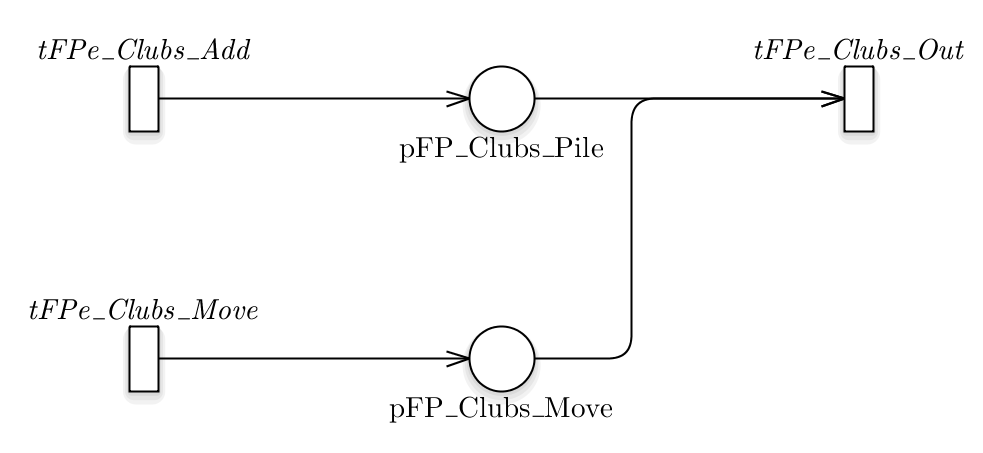
\includegraphics[width=\textwidth]{images/foundationPile}
		\caption{Foundation Pile Module}
	\end{center}

bla bla bla
\end{figure}

\begin{table}
	\caption{Transitions used in Foundation Piles}
	\begin{tabular}{|l|l|l|}
		\hline
		& Name & Description \\
		\hline
		9  & tFPe\_Clubs\_Add         &    \\ \hline
		10 & tFPe\_Clubs\_Move        &    \\ \hline
		11 & tFPe\_Clubs\_Out         &    \\ \hline
		12 & tFPe\_Diamonds\_Add      &    \\ \hline
		13 & tFPe\_Diamonds\_Move     &    \\ \hline
		14 & tFPe\_Diamonds\_Out      &    \\ \hline
		15 & tFPe\_Hearts\_Add        &    \\ \hline
		16 & tFPe\_Hearts\_Move       &    \\ \hline
		17 & tFPe\_Hearts\_Out        &    \\ \hline
		18 & tFPe\_Spades\_Add        &    \\ \hline
		19 & tFPe\_Spades\_Move       &    \\ \hline
		20 & tFPe\_Spades\_Out        &    \\ \hline
	\end{tabular}
\end{table}
\begin{table}
	\caption{Places used in Foundation Piles}
	\begin{tabular}{|l|l|l|}
		\hline
		& Name & Description \\
		\hline
		7  & pFP\_Clubs\_Move          &  \\ \hline
		8  & pFP\_Clubs\_Pile          &  \\ \hline
		9  & pFP\_Diamonds\_Move       &  \\ \hline
		10 & pFP\_Diamonds\_Pile       &  \\ \hline
		11 & pFP\_Hearts\_Move         &  \\ \hline
		12 & pFP\_Hearts\_Pile         &  \\ \hline
		13 & pFP\_Spades\_Move         &  \\ \hline
		14 & pFP\_Spades\_Pile         &  \\ \hline
	\end{tabular}
\end{table}
\subsection{Tableau Pile Module}

\begin{figure}
	\begin{center}
		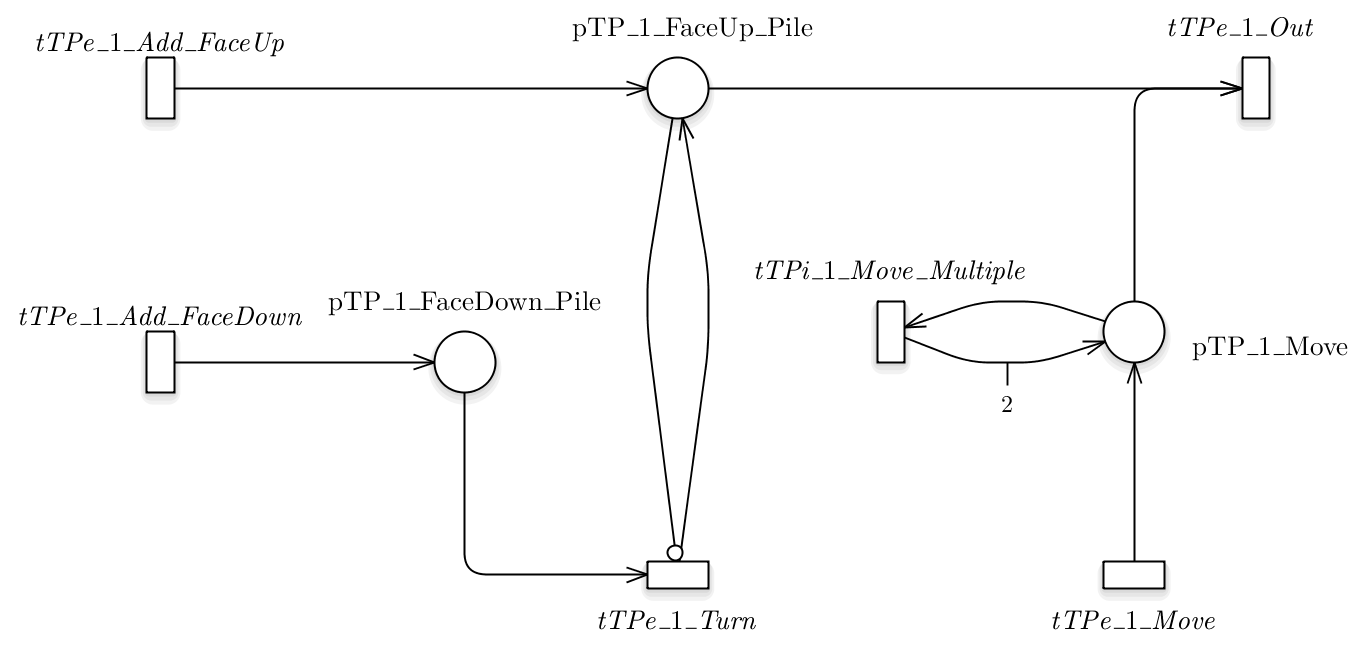
\includegraphics[width=\textwidth]{images/tableauPile}
		\caption{Tableau Pile Module}
	\end{center}
\end{figure}
\begin{table}
	\caption{Transitions used in Tableau Piles}
	\begin{tabular}{|l|l|l|}
		\hline
		& Name & Description \\
		\hline
		53 & tTPe\_1\_Add\_FaceDown   &    \\ \hline
		54 & tTPe\_1\_Add\_FaceUp     &    \\ \hline
		55 & tTPe\_1\_Move            &    \\ \hline
		56 & tTPe\_1\_Out             &    \\ \hline
		57 & tTPe\_1\_Turn            &    \\ \hline
		58 & tTPe\_2\_Add\_FaceDown   &    \\ \hline
		59 & tTPe\_2\_Add\_FaceUp     &    \\ \hline
		60 & tTPe\_2\_Move            &    \\ \hline
		61 & tTPe\_2\_Out             &    \\ \hline
		62 & tTPe\_2\_Turn            &    \\ \hline
		63 & tTPe\_3\_Add\_FaceDown   &    \\ \hline
		64 & tTPe\_3\_Add\_FaceUp     &    \\ \hline
		65 & tTPe\_3\_Move            &    \\ \hline
		66 & tTPe\_3\_Out             &    \\ \hline
		67 & tTPe\_3\_Turn            &    \\ \hline
		68 & tTPe\_4\_Add\_FaceDown   &    \\ \hline
		69 & tTPe\_4\_Add\_FaceUp     &    \\ \hline
		70 & tTPe\_4\_Move            &    \\ \hline
		71 & tTPe\_4\_Out             &    \\ \hline
		72 & tTPe\_4\_Turn            &    \\ \hline
		73 & tTPe\_5\_Add\_FaceDown   &    \\ \hline
		74 & tTPe\_5\_Add\_FaceUp     &    \\ \hline
		75 & tTPe\_5\_Move            &    \\ \hline
		76 & tTPe\_5\_Out             &    \\ \hline
		77 & tTPe\_5\_Turn            &    \\ \hline
		78 & tTPe\_6\_Add\_FaceDown   &    \\ \hline
		79 & tTPe\_6\_Add\_FaceUp     &    \\ \hline
		80 & tTPe\_6\_Move            &    \\ \hline
		81 & tTPe\_6\_Out             &    \\ \hline
		82 & tTPe\_6\_Turn            &    \\ \hline
		83 & tTPe\_7\_Add\_FaceDown   &    \\ \hline
		84 & tTPe\_7\_Add\_FaceUp     &    \\ \hline
		85 & tTPe\_7\_Move            &    \\ \hline
		86 & tTPe\_7\_Out             &    \\ \hline
		87 & tTPe\_7\_Turn            &    \\ \hline
		88 & tTPi\_1\_Move\_Multiple  &    \\ \hline
		89 & tTPi\_2\_Move\_Multiple  &    \\ \hline
		90 & tTPi\_3\_Move\_Multiple  &    \\ \hline
		91 & tTPi\_4\_Move\_Multiple  &    \\ \hline
		92 & tTPi\_5\_Move\_Multiple  &    \\ \hline
		93 & tTPi\_6\_Move\_Multiple  &    \\ \hline
		94 & tTPi\_7\_Move\_Multiple  &    \\ \hline
	\end{tabular}\end{table}
\begin{table}
	\caption{Places used in Tableau Piles}
	\begin{tabular}{|l|l|l|}
		\hline
		& Name & Description \\
		\hline
		22 & pTP\_1\_FaceDown\_Pile    &  \\ \hline
		23 & pTP\_1\_FaceUp\_Pile      &  \\ \hline
		24 & pTP\_1\_Move              &  \\ \hline
		25 & pTP\_2\_FaceDown\_Pile    &  \\ \hline
		26 & pTP\_2\_FaceUp\_Pile      &  \\ \hline
		27 & pTP\_2\_Move              &  \\ \hline
		28 & pTP\_3\_FaceDown\_Pile    &  \\ \hline
		29 & pTP\_3\_FaceUp\_Pile      &  \\ \hline
		30 & pTP\_3\_Move              &  \\ \hline
		31 & pTP\_4\_FaceDown\_Pile    &  \\ \hline
		32 & pTP\_4\_FaceUp\_Pile      &  \\ \hline
		33 & pTP\_4\_Move              &  \\ \hline
		34 & pTP\_5\_FaceDown\_Pile    &  \\ \hline
		35 & pTP\_5\_FaceUp\_Pile      &  \\ \hline
		36 & pTP\_5\_Move              &  \\ \hline
		37 & pTP\_6\_FaceDown\_Pile    &  \\ \hline
		38 & pTP\_6\_FaceUp\_Pile      &  \\ \hline
		39 & pTP\_6\_Move              &  \\ \hline
		40 & pTP\_7\_FaceDown\_Pile    &  \\ \hline
		41 & pTP\_7\_FaceUp\_Pile      &  \\ \hline
		42 & pTP\_7\_Move              &  \\ \hline
	\end{tabular}
\end{table}
\subsection{Module Connector Module}

\subsection{Player Module}

\subsection{Player Bot Module}


\section{Implementation}
\label{sec:3_implementation}
\subsection{\ac{gui}}
\label{sec:3_gui}
\subsection{Algorithms}
\subsubsection{Atomicity}
\subsection{Commands}
In order to preventdd
\subsection{Initial Dealing}
\subsection{Resources}
\label{sec:3_Resources}
\subsection{Moving Multiple Cards}
\subsection{Scoring}
\subsection{Possible improvments}
A major drawback of the siphon \verb!tMC_Out_Buffer_Siphon! is that if it fires, the card will actually be removed from the game, and the game becomes unsolvable. This transition will fire if the move-command of the token has an invalid destination. Due to how the Player and Player Bot modules are set up, this will never happen as they will check the validity of the move command before actually issuing the command. Still, I think it would be an improvement add an additional transition to the Draw Pile module which would accept cards from \verb!tMC_Out_Buffer_Siphon!, instead of totally discarding them.
\newline

Another improvement would be to refactor the codebase by moving more of the validity check of the commands from the Player and Player Bot modules to the destination transitions. The Player Bot modules uses roughly 200 lines of code to always issue valid commands, I think this could be drastically reduced. By doing this it would be easier to create additional modules which could interface with the game, for example a hardware-based module.

\begin{verbatim}
    def mapper_from_to(self, key, email):
        if 'to' in email.keys() and 'from' in email.keys() and 'body_count' in email.keys():
\end{verbatim}

\section{Testing, Analysis and Results}
\label{sec:3_testing_analysis}
\subsection{Algorithms}
\subsubsection{Atomicity}
In order to preventdd
\subsection{Initial Dealing}
\subsection{Resources}
\subsection{Moving Multiple Cards}

\section{Discussion}



% Keeping this for reference for now %
\begin{thebibliography}{6}

\bibitem{wikiTFIDF} Wikipedia article on Tf-idf. \url{https://en.wikipedia.org/wiki/Tf?idf}
\bibitem{oreilly} Tom White, Hadoop: The Definitive Guide, 2015, \emph{ISBN: 978-1-491-90163-2}
\bibitem{dockerdocs} Docker API Docs, \url{https://docs.docker.com}
\bibitem{dat630slides} Slides from DAT630, Krisztian Balog
\bibitem{dataset} Kaggle. The Enron Email Dataset. \url{https://www.kaggle.com/wcukierski/enron-email-dataset}
\bibitem{coursematerial} Data Intensive Systems Compendium, Tomasz Wiktorski et al.

\end{thebibliography}

\end{document}
